
\documentclass[a4paper,11pt]{report}

\usepackage{amsmath,amssymb,amsfonts,amsthm}    	% Typical maths resource packages

\usepackage{url}									% Enter URL like \url{...}
\usepackage{hyperref}                           	% For creating hyperlinks in cross references

\usepackage{listings}                           	% Packages to allow inclusion of lists
\usepackage{rotating}                           	% Packages to allow rotations

\usepackage{multicol,multirow}                   % Packages to allow multi collum / row text
\usepackage{geometry}							% See geometry.pdf to learn the layout options. There are lots.
%\geometry{landscape}							% Activate for for rotated page geometry
\usepackage[parfill]{parskip}        			% Activate to begin paragraphs with an empty line rather than an indent
%\usepackage{epstopdf}							% eneables use of eps with PDFtoLatex
\usepackage{float}								% use big tables, figures broken by page-change
%\floatstyle{style: plained, plaintop, boxed, ruled)} % Specification for sutom float style
%\newfloat{type}{placement}{ext}[outer counter]	% Specification for sutom float style

%--- Encodings & Fonts ---
\usepackage[utf8]{inputenc}						% Input Encodings of the used Editor
\usepackage[T1]{fontenc}							% font encoding (e.g. for textcopy out of PDFs)
\usepackage{textcomp}							% for special characters like (degree, euro-symbol, greek-symbols, ..)
%\usepackage{verbatim}							% "wörtlich" writes with /begin and /end verbatim paragraphes in normal form
\usepackage{alltt}								% as verbatim but slightly different
%\usepackage{color}								% Enable use of colored texts


%--- Abreviations ---
\usepackage[nomain,acronym,xindy,toc]{glossaries} % nomain, if you define glossaries in a file, and you use \include{INP-00-glossary}
\makeglossary

%--- Figures, Captions, Labels ---
%\usepackage[bf]{caption2}
\usepackage{subfig}								% enables small figures order within one header figure
\usepackage{graphicx}                           	% Packages to allow inclusion of graphics
\usepackage{wrapfig}								% Use to wrap text aroud images


%--- Language ---
\usepackage[german]{babel}


%--- citation and literature ---
\usepackage[round]{natbib}						% literature reference style --> round mean author,year citation style!


%--- define topline ---
\usepackage[automark]{scrpage2}
\pagestyle{scrheadings}
\automark{section}
\clearscrheadings
\ohead{\headmark}
\cfoot{\pagemark}


%--- define page size, margin size ---
\setlength{\headheight}{1.1\baselineskip}
\voffset=-3cm
\hoffset=-3cm
\textheight24cm
\textwidth16.5cm
\topmargin1cm
\oddsidemargin3cm
\evensidemargin3cm

% define line line spacing = 1.5
\renewcommand{\baselinestretch}{1.5}

% define second level for `itemizing'
\renewcommand{\labelitemii}{-}

% --------------------------------------
% --------------------------------------

\begin{document}

% -------------------------------
% --- frontmatter: Title page ---
% -------------------------------
\thispagestyle{empty}

\begin{center}
\vspace*{\fill}

    {\Large{\bf Concept of an mobile assisting system for multi-sensor buildings-observation}} \vspace{0.5cm}
    
    {\Large{Entwurf eines mobiles Assistenzssystem für multisensorische Bauwerksüberwachung}} \vspace{0.5cm}


    {\normalsize EXPOSE: Master Thesis Euteneuer}\\\vspace{0.5cm}
    {\normalsize Technische Universität Berlin \\
    Institute für Geodäsie und Geoinformationstechnik\\
	Fachgebiet Methodik der Geoinformationstechnik\\
	superviesd by:\\	
	Prof. Frank Neitzel\\
	Thomas Becker}\vspace{1cm}

    {\normalsize by \\\vspace{0.5cm}
    {\bf Frieder H. Euteneuer}} \vspace{1cm}
		

    {\normalsize Berlin, \today}
\vfill
\end{center}




% ------------------------------------
% --- frontmatter: Acknowledgement ---
% ------------------------------------
\newpage
\pagenumbering{roman}   % define page number in roman style
\setcounter{page}{1}    % start page numbering
%\input{acknowledgement}

% -----------------------------
% --- frontmatter: Abstract ---
% -----------------------------
%\newpage
%\input{abstract}



% -----------------------------
% --- frontmatter: Contents ---
% -----------------------------
\newpage
\tableofcontents
%\clearpage


% ----------------------------------------------------
% --- frontmatter: List of Figures (not mandatory) ---
% ----------------------------------------------------
\newpage
\addcontentsline{toc}{section}{Abbildungsverzeichnis}
\ohead[]{\rightmark}
\listoffigures


% ---------------------------------------------------
% --- frontmatter: List of Tables (not mandatory) ---
% ---------------------------------------------------
\newpage
\addcontentsline{toc}{section}{Tabellenverzeichnis}
\listoftables

\newpage
\printglossary[title=Akronyme]



% -------------------------------
% --- main body of the thesis ---
% -------------------------------
\newpage
\setcounter{page}{1}    								% start page numbering anew
\pagenumbering{arabic}  								% page numbers in arabic style
\setcounter{secnumdepth}{4}


\part{Einleitung und Motivation}
-This chapter will describe how the system will be designed, how the Field of application can be modelled, what functionalities can be planned-

\section{Einsatzgebiet}
Um präzise beschreiben zu können was das System tun können muss, ist es notwendig vorher konkret die vorliegende Situation oder das existierende Problem zu definieren. Solche eine Definition sollte eine Beschreibung der Umgebung beinhalten in der das System eingesetzt werden soll. Nimmt man eine Modellierungssprache zur Hilfe, um die Umgebung zu beschrieben, ist es später einfacher daraus Rückschlüsse auf mögliche Probleme zu ziehen. Für ein solches Modell müssen die Fragen beantwortet werden, in welche Objekte sich die Umgebung aufgliedert, wie diese interagieren und welche Funktionalitäten diese dafür verwenden.Aber auch die teilhabenden Akteure und ihre konkreten Anforderungen an das System müssen modelliert werden. Mit Hilfe von exemplarischen Anwendungsfällen werde ich beschreiben was der tatsächliche Bedarf des Nutzers ist, und wie dieser gedeckt werden kann.

Bevor ich mit dem technischen Ausformulieren der Modellierung beginne, möchte ich kurz in die Thematik einleiten: Das System welches ich mit dieser Arbeit konzeptioniere soll Feldingenieuren helfen im Feld mit den Messungen und Daten verschiedener Sensoren zu arbeiten. Als konkretes Beispiel werde ich den Einsatz des Systems bei der Bauwerksüberwachung mithilfe eines Sensornetzwerkes beschreiben.

Die Überwachung von Bauwerken mittels eines Netzwerkes aus verschiedenen Sensoren hilft ihre Sicherheit ohne den Einsatz großer Bautechnischer Überprüfungen einschätzen zu können. Damit ist es möglich Bauwerke auch weit über ihre geplante Lebensdauer hinweg zu erhalten. Ohne den Einsatz solcher Sensor Netzwerke können die zuständigen Gutachter bei Ablauf der geplanten Lebensdauer nicht darauf vertrauen, dass das Gebäude auch weiterhin den kontinuierlichen Belastungen gewachsen ist, und somit werden entweder umfangreiche Sanierungen Nötig, oder Gebäude werde geschlossen. Die Überwachung basiert auf der Messung von Veränderungen von verschiedenen Parametern wie zum Beispiel der Position , der Temperatur oder Feuchtigkeit von Bauteile oder der Abweichungen von charakteristischen Bewegungsmustern von Bauteilen, gemessen durch Beschleunigungssensoren. Die Parameter werden sowohl punktuell  verteilt über das gesamt Bauwerk, als auch gesamtheitlich die Struktur des Bauwerkes miteinbeziehend erhoben, siehe auch \citep{worden_overview_2004} \citep{farrar_introduction_2007} \citep{boller_structural_2004}. Für die Messungen werden zum einen automatisch kontinuierlich messende Systeme eingesetzt, und zum anderen seltenere manuelle Messungen, deren Ergebnisse manuelle in das System eingegeben werden. 

Für das bessere Verständnis möchte ich hier ein Beispielfall beschreiben: Ein Brücke erreicht ihre letzten Jahre der Betriebserlaubnis. Danach müssen entweder die Verkehrssicherheit erneut umfangreich geprüft, und zahlreiche Verschleißteile, deren Zustand schlecht zu beurteilen ist, ersetzt werden, oder die Verkehrssicherheit muss auf andere Art überprüft werden. Zahlreiche Sensoren werden an den einzelnen wichtigen Gebäudeteilen eingerichtet, und überwachen nun automatisch über einen bestimmten Zeitraum deren Verhalten und Veränderungen. In periodischen Abständen werden automatisch Diagnosen erstellt, basierend auf der Analyse der Messwerte, der Überprüfung des Materialverschleißes und einiger anderer Einflussgrößen. Eine detailliertere Beschreibung der verwendeten Messungen, Zeitskalen und Analysemethoden werden in den nachfolgenden Kapiteln beschrieben.

In der Einleitung der Arbeit möchte ich mich am Verlauf der Erstellung eines Pflichtenheftes für die Softwareentwicklung orientieren , da so am besten modelliert werden kann wie der Bedarf des Nutzers gedeckt werden kann, siehe auch \citep{gregor_engels_vorlesung_2006}. Beginnen werde ich mit einer textuellen Beschreibung der Situation. Danach folgt eine Modellierung der Prozesse und der Akteure mit ihren jeweiligen Anwendungsfällen. Zum Abschluss werde ich dann die daraus abgeleiteten notwendigen Funktionalitäten des System beschreiben.


\subsection{Modell des Problembereichs}
Die Abbildung \ref{fig:model_domain} zeigt ein UML Diagramm (Unified Modeling Language) das die im folgenden beschrieben verschiedenen Objekte des Systems beinhaltet. Das Modell beschreibt die Beziehungen der einzelnen Objekte untereinander und modelliert keine Aktivitäten oder Funktionen.

Die Umgebung in der das System eingesetzt werden wird besteht aus fünf verschiedenen Arten von Objekten und deren Beziehungen untereinander. Zentrales Objekt ist der Daten Server, der als Knoten für die Kommunikation zwischen den einzelnen Kompartimente dient. Diese sind hauptsächlich die Sensoren selbst, die jedoch ohne einen Server, der als Steuerungseinheit für jeden Sensor dient, nicht selbständig messen können. Der Server kontrolliert die Sensoren indem er sie aktiviert und deaktiviert. Nichtsdestotrotz können Sensoren in einem separiertem eigenem Netzwerk organisiert sein, das dann wiederum als einzelner Sensor behandelt wird. Die Sensoren senden ihre gemessenen Daten entweder aktiv an den Server beziehungsweise über den Server an die dem Server angeschlossene Datenbank, oder der Server ruft die Daten aktiv ab, und speichert diese dann in der Datenbank.

\begin{figure}[H]
	\centering
 	 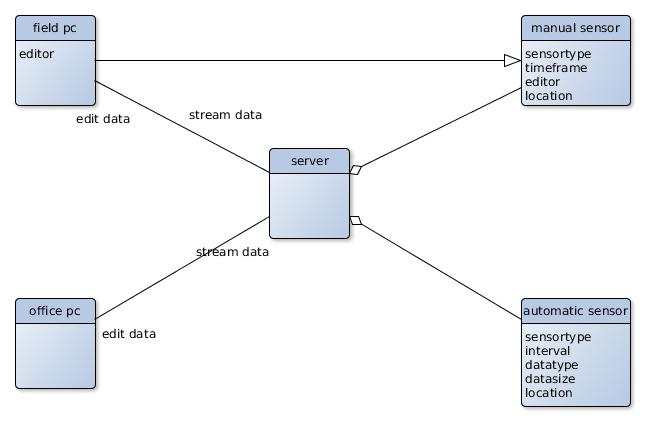
\includegraphics[scale=0.6]{graphics/model_of_issue.jpg} 
	\caption{Modell des Problembereiches mit relevanten Objekten, F. H. Euteneuer 2013}
	 \label{fig:model_domain}
\end{figure}

Die Datenbank die and den Server angeschlossen ist speichert sowohl Metadaten zu den Sensoren, als auch die gemessenen Werte. Unter Metadaten sind alle Informationen zu verstehen, die die Sensoren eindeutig beschreiben, und die für weitere Analysen der Messerwerte erforderlich sind (siehe auch im Glossar "Metadaten". Beispielsweise sind das die Positionen der Sensoren, die Messintervalle, die Sensortypen oder die übermittelten Datentypen.

Als Klient des Services kann im Prinzip jede Art von mobilen Systemen eingesetzt werden. Angeschlossen an die Datenbank dienen diese dann als bildgebender Teil des Systems. Da die Verknüpfung mit einem Server meist über das Protokoll TCP/IP geschieht, müssen mobile Geräte über eine Internetverbindung verfügen. Die Verwendung dieser Geräte bleibt dadurch begrenzt auf Gebiete innerhalb der Handynetz-Abdeckung. Für manuelle Messungen dient der mobile Klient zusätzlich als Eingabegerät für die Messwerte, sofern dies nicht über das Gerät selber erfolgen kann. Dadurch wird der mobile Klient in dem Modell sowohl als bildgebender Teil des Systems, als auch als Sensor behandelt, und ererbt damit die Eigenschaften des Sensor Objekts.

Das System will einen ganzheitlichen Ansatz verfolgen, und beinhaltet somit auch einen Teil der für die umfangreicheren Analysen zuständig ist, sowie durch eine Datenexportfunktion als Schnittstelle zu weiteren Algorithmen und System dient. Dieser Teil des System wird in dem Modell durch den "Desktop-Computer" repräsentiert. Die eigentliche Einrichtung und Planung des Systems wird erwartungsgemäß von diesem, dem bequemeren Arbeitsplatz (verglichen mit dem mobilen Klienten), durchgeführt werden. Zusätzlich zu den Eigenschaften des Feldcomputers sind somit erweiterte Verwaltungs- und Analysefunktionen als Eigenschaften dieses Objektes definiert.


\subsection{Geschäftsprozesse}
Wichtigste Entscheidungshilfe für die Nutzung solch eines Systems wird die Eigenschaft des Systems, eine entscheidungsunterstützende Funktion zu erfüllen, sein. Das System ist fokussiert auf die wichtigen Werkzeuge die die Arbeit des Feldingenieurs vereinfachen sollen, und lässt unwichtige oder komplizierte Werkzeuge komplett weg. Außerdem werden die Informationen die im Feld auf dem mobilen Klienten angezeigt werden derart reduziert, dass lediglich aussagekräftige Werte, die damit Entscheidungen unterstützen können, angezeigt werden. In dem vorherigem Kapitel habe ich den Problembereich beschrieben, nun möchte ich die verschiedenen Prozesse skizzieren die ein Nutzer durchführen könnte.

\begin{figure}[H]
	\centering
 	 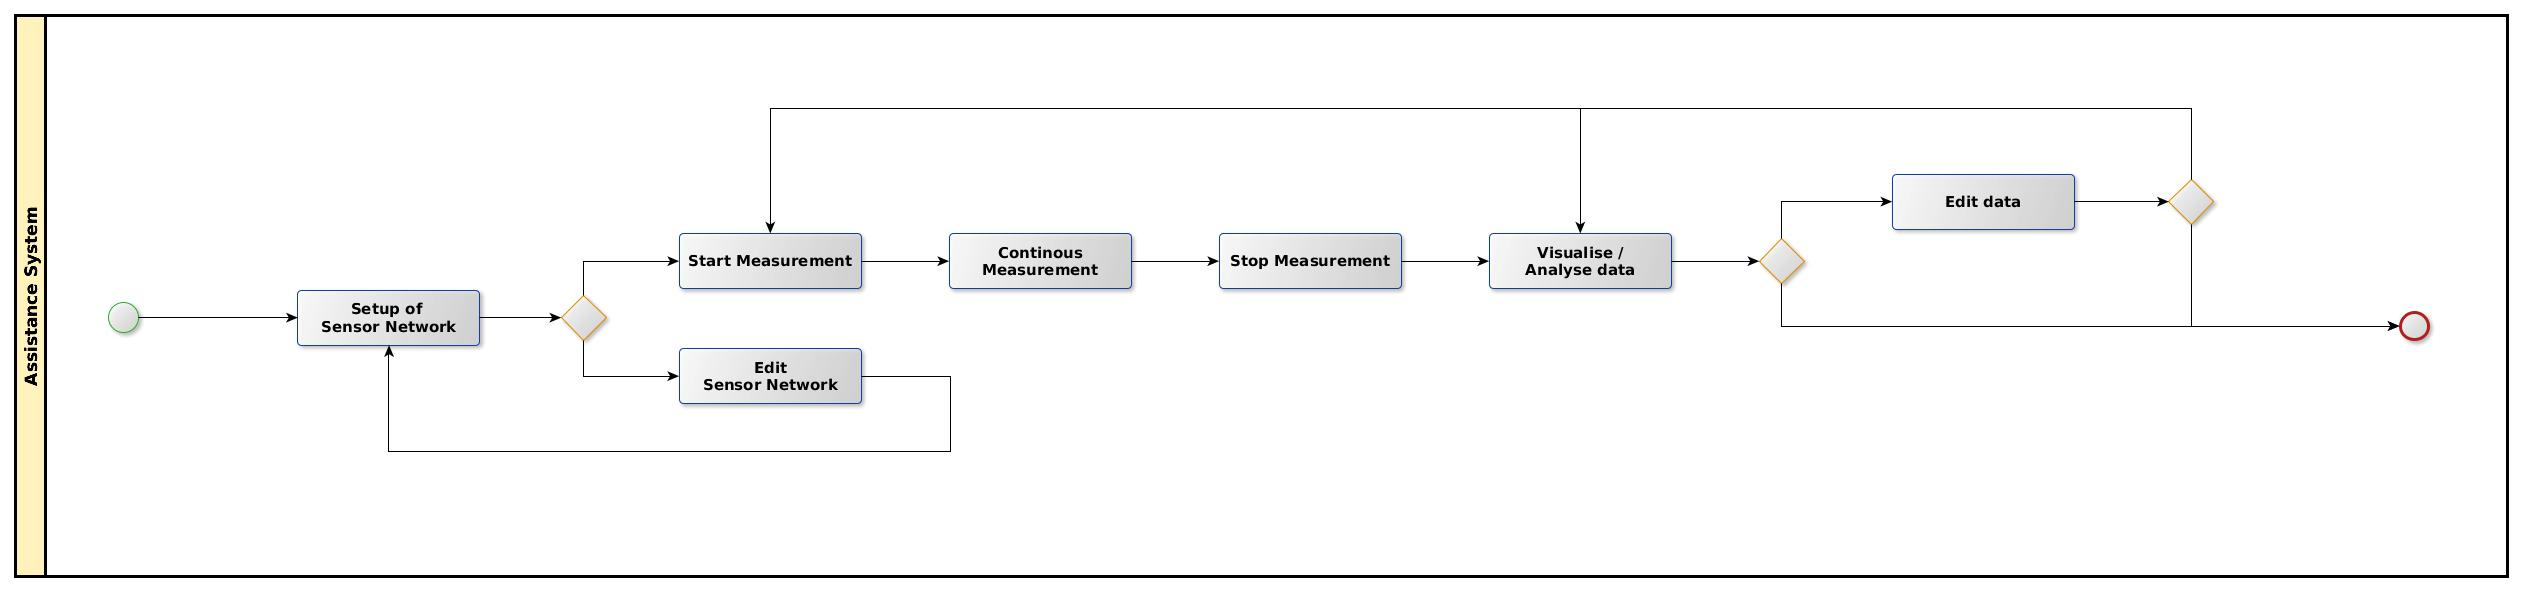
\includegraphics[scale=0.2]{graphics/bpmn_business-processes.jpg} 
	\caption{BPMN (Business Process Model and Notation) Modell relevanter Aktionen welche in dem System durchgeführt werden, F. H. Euteneuer 2013}
	 \label{fig:model_business-processes}
\end{figure}

Ich habe drei verschiedene Hauptaktionen identifiziert, die ein Nutzer durchführen könnte: Das manuelle Messen von Werten, das manuelle Editieren bereits gemessener Werte, und das automatische kontinuierliche Messen. Die Abbildung \ref{fig:model_business-processes} veranschaulicht mittels eines UML Activity Diagrams (UML Aktivitäten Diagramm) die einzelnen Abläufe dieser Aktionen.

Die manuelle Messung beginnt mir der normalen Messung der Werte. Im zweiten Schritt erfolgt die Eingabe der Werte in das System. Die Werte werden automatisch auf ihre Validität hin überprüft, und erste einfache statistische Analysen werden erstellt. Diese erste Statistik ist erforderlich um Informationen über die Qualität der Messung zu erhalten, und dem System die Möglichkeit zu bieten fehlerhafte Messungen zu bemängeln und Neumessungen vorzuschlagen.

Der Nutzer wird die Möglichkeit haben vergangene Messungen manuell zu bearbeiten. Dazu muss ein Datensatz (Üblicherweise ein Messwert) ausgewählt werden, und der Nutzer kann dann entscheiden ob die betreffende Messung wiederholt werden soll, oder die Werte manuell geändert werden sollen. Bei einer Wiederholung der Messung wird die Prozesskette der manuellen Messung durchlaufen.


The automatic measurements are the most important one for the described SHM. The will be the backbone of the system, nevertheless they are using similar functionalities. The user will initially be able to set the sensor network up. Which means to enter metadata about the used sensors like position, reference system, type of sensor, measurement interval, etc. A more detailed description of what is needed for such a setup will follow in the methodical part. After the setup, the user is able to start the measurements with the defined parameter, or the edit the settings.

As a conclusion of this chapter, I would like to point out that this list is only representing functionalities of a basic system, and should not be understood as being complete.


\section{Functionalities}
This chapter will describe what the system should provide to solve the problem and/or make the existing situation better: Which functionalities should be part of the system. To get closer to a possible solution, the different stakeholders and their use cases in the domain of structural health monitoring must be defined and described.

\begin{figure}[H]
	\centering
 	 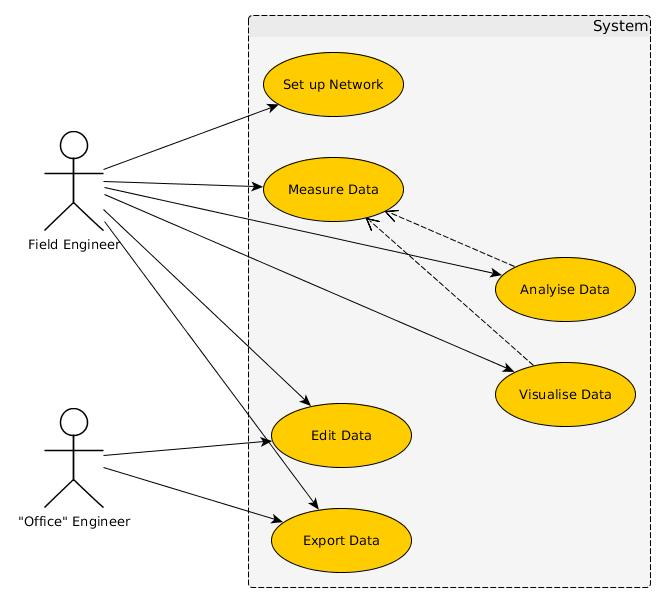
\includegraphics[scale=0.6]{graphics/uml_functionalities.jpg} 
	\caption{UML Use Case Diagram of the described System describing two different users and their use cases. By F. H. Euteneuer 2013}
	 \label{fig:model_functionalities}
\end{figure}

\subsection{Usergroups}
As a main source for information and parameter for the concept of a software, the usergroups are of large importance. I will analyse the involved usergroups and their needs respective expectations to get those information. As the figure \ref{fig:model_functionalities} is already representing, I have identified two main usergroups which might be involved in the processes.

\subsubsection{Field-engineer}
The group of field-engineers can described as the executive persons which are dealing with the direct measurements, observations and setup of an automatic measurement network. This group can be categorised by its technically limits, which are:
\begin{itemize}
\item the small screen-size of the mobile computers (quality of visualisation is limited)
\item the lack of input facilities (e.g. only digital keyboard on a handheld computer)
\item high weight of not handheld instruments (e.g. a conventional laptops too heavy for using while walking/standing)
\end{itemize}
But nevertheless, this usergroup has the most challenging requirements on the system when speaking about visualisation options or analysis computation in advance. It is the central target usergroup for this system, therefore it should fit mostly to its requirements.


\subsubsection{Office-engineer}
Usually the field-engineer and the office-engineer are combined in one person. One part of an observation project is dealing with the field-work, the setup, measurements and maintenance. And the other part is the precise analysis of the data, the post processing and its interpretation. Due to a high quality equipment in the offices, this part is mostly better solvable for a software. Here does not the system has to be restricted by the environment, but the system is making its demands on the technical environment.


\subsection{Use Cases}
The Figure \ref{fig:model_functionalities} is showing the different basic use cases of the described two usergroups. Use cases shown in this figure are representing activities of the user which have to be complete with it own defined target. I want now describe the use cases in detail with further parameter. This is important for the further proceeding of the system conception, because use cases are defining the users interests of a system.

The following part will describe the selected use cases in detail. All the use cases will be described with tables for the textual description which are containing information about the use case goal, the postcondition and further more. For the description of the the chronological task flow of the use cases also a activity diagram will depict each use case.

Important to know is, that the diagrams are not representing all possible activity flows which are available. They are representing one possible option which could solve the problem and will be implemented in the prototype.

The use cases are divided into three different groups. There are use cases dealing with central data management functionalities, others are describing main measurement functionalities and the last are describing the data analysis functionalities.


\subsubsection{Management}
There are several use cases with central management functionalities of the system. Management stands for both, data management and system management.  

First use case within the system is the setting up of the network. It can be understood as the initial task and therefore a kind of a precondition for all other use cases.The table \ref{table:use case description of "Set up network"} is describing central features of this use case. 

The export of the data is another major task within the management field. It could be denoted as the final task interacting with the system. The second table \ref{table:use case description of "Export data"} is showing detailed information about the "Export data" use case.

\begin{table}[H]
\centering
\begin{tabular}{l | p{11cm}}
Name & Set up network\\ \hline 
Usergroup & Field engineer\\ \hline 
Goal & Input all metadata about connected sensors and initialise network\\ \hline 
Precondition & Network physically existing and able to correspond with system\\ \hline 
Postcondition & working network with all sensors\\ 
\end{tabular}
\caption{Use Cases tabular description of characteristics} 
\label{table:use case description of "Set up network"}
\end{table}

\begin{table}[H]
\centering
\begin{tabular}{l | p{11cm}}
Name & Export data\\ \hline 
Usergroup & Office Engineer\\ \hline 
Goal & Specify data by parameter and specify output format\\ \hline 
Precondition & Specified data and output format\\ \hline 
Postcondition & complete dataset in specific format offline\\ 
\end{tabular}
\caption{Use Cases tabular description of characteristics} 
\label{table:use case description of "Export data"}
\end{table}

Figure \ref{fig:bpmn_use-case_management} is showing the systems management use cases in a two line activity diagram. The both activity flows do not have any interaction in between, but chronologically must the setup use case performed before the export use case.

The activity flow of the setup use case is showing two main tasks: The database-setup and the input of the sensor-parameter. Those are the central parts and their success or failure is leading to an overall success or failure. An edit of an existing network is leading to a restart of the full procedure. This could be interpreted as an assistant which is leading through the different configurations and is taking care of possible errors.

The export use case is much easier, it is simply the normal flow which is equal to most of the download assistants which can be found online. The only important information about that is the determination of the export datasets time-frame.

\begin{figure}[H]
	\centering
 	 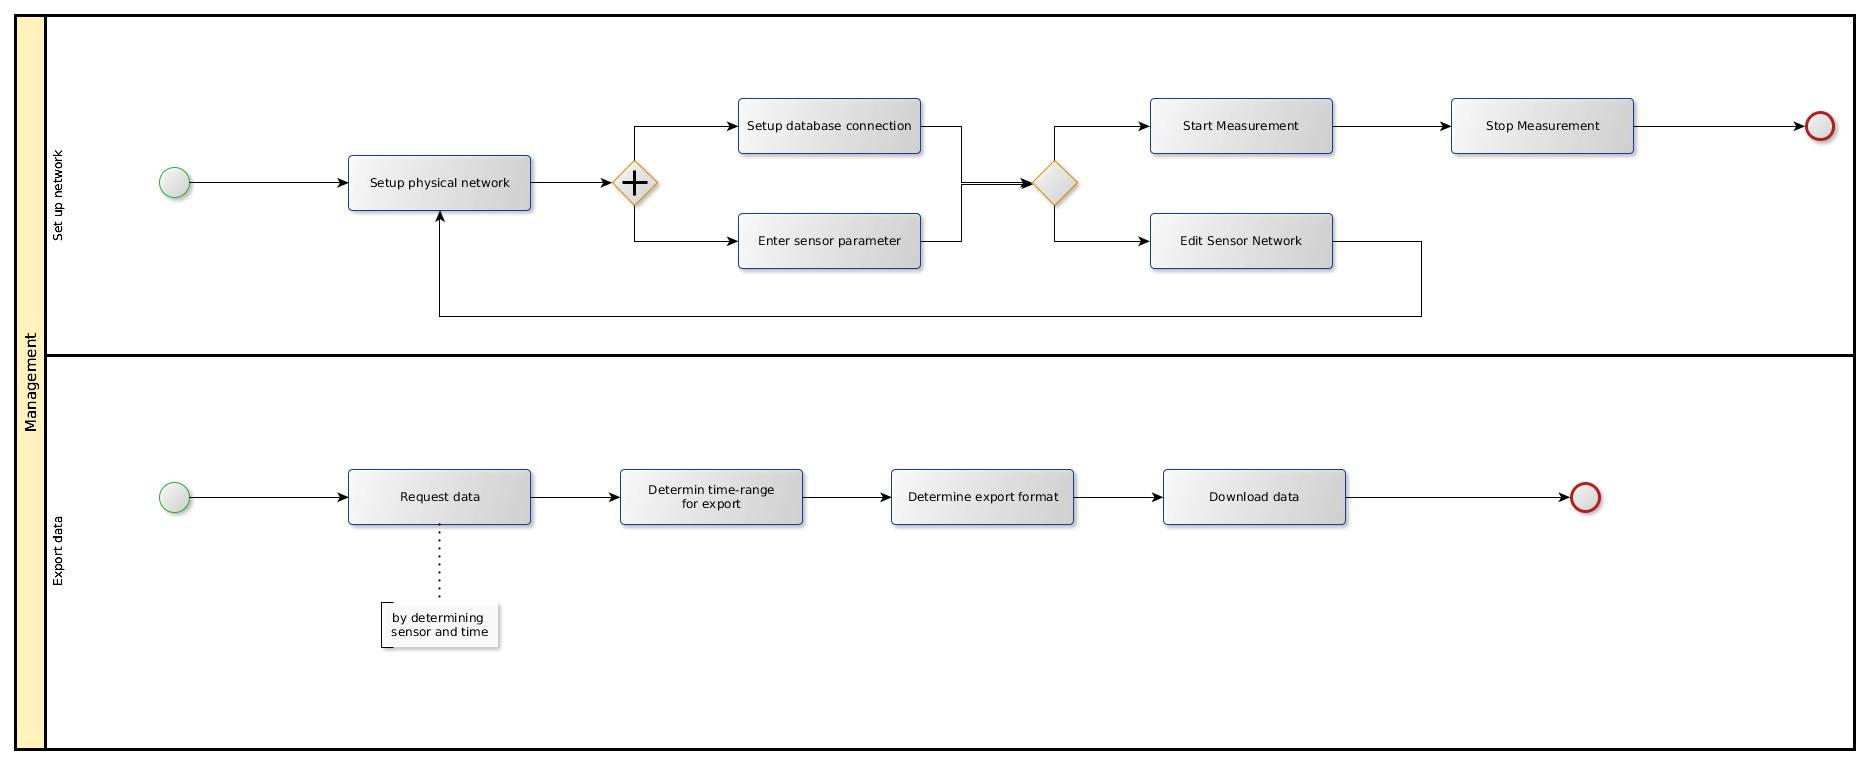
\includegraphics[scale=0.24]{graphics/bpmn_use-cases_management.jpg} 
	\caption{BPMN (Business Process Model and Notation) Model of the use cases describing central management proceedings. By F. H. Euteneuer 2013}
	 \label{fig:bpmn_use-case_management}
\end{figure}


\subsubsection{Measuring}

The measurement part might be the most important one within the system. This part is the only one which is describing a manual manipulation of the data in the database.

There are two identified use cases: The first is dealing with the initial data input which is the measurement see table \ref{table:use case description of "Measure data"}. In contrast to the automatic measurements, this is describing a discrete manual measurement, and the input of the data by hand.

And the second one is editing already existing data in the database see table \ref{table:use case description of "Edit data"}. This is a merely a standard operation for database related systems. Nevertheless, this task is related to the measurement task, in case of re-measuring data or validation of data.

\begin{table}[H]
\centering
\begin{tabular}{l | p{11cm}}
Name & Measure data\\ \hline 
Usergroup & Field engineer\\ \hline 
Goal & Input all data by hand  getting from standalone measurement device\\ \hline 
Precondition & Running system and access to database\\ \hline 
Postcondition & valid data in the database with full set of metadata\\ 
\end{tabular}
\caption{Use Cases tabular description of characteristics} 
\label{table:use case description of "Measure data"}
\end{table}

\begin{table}[H]
\centering
\begin{tabular}{l | p{11cm}}
Name & Edit data\\ \hline 
Usergroup & Office Engineer\\ \hline 
Goal & Specify data by parameter and input new values by hand or measurement\\ \hline 
Precondition & Running system and access to database\\ \hline 
Postcondition & changed data in the database with full set of metadata\\ 
\end{tabular}
\caption{Use Cases tabular description of characteristics} 
\label{table:use case description of "Edit data"}
\end{table}

When performing a manual measurement, most of the task described in the first line of the figure \ref{fig:bpmn_use-case_measuring} will be mandatory tasks. In the end the system will perform a quick analysis of the inserted data in order to validate the measurement. After this step the system will either point out possible errors, or it will approve the measurements, and write them into the database. The second line, the editing flow, is offering two options, one is a manual insert of new data, another would lead to a re-entering of the manual measurement flow, in order to overwrite the selected datasets with new measurements.

\begin{figure}[H]
	\centering
 	 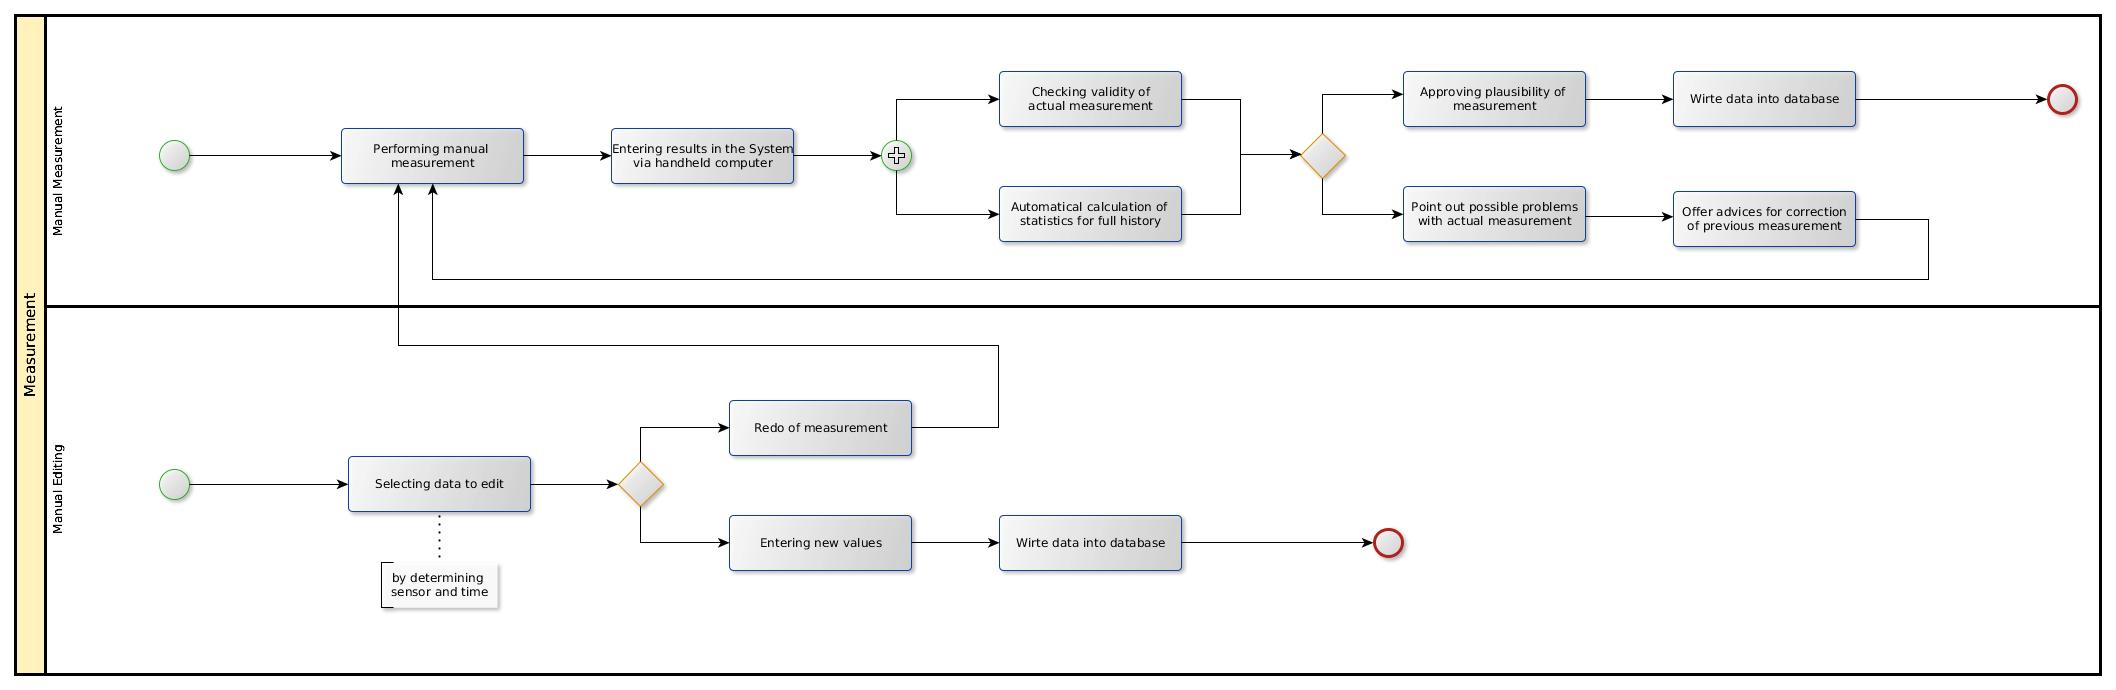
\includegraphics[scale=0.24]{graphics/bpmn_use-cases_measurement.jpg} 
	\caption{BPMN (Business Process Model and Notation) Model of the use cases describing central measuring proceedings. By F. H. Euteneuer 2013}
	 \label{fig:bpmn_use-case_measuring}
\end{figure}

\subsubsection{Analysis}

A complex part is the analysis functionalities of the system which will be described in this section. The analysis described here will be slightly different to the "ad hoc" statistics in the previous part which are leading to approved or discarded measurements. Those are checking the coherence of the performed measurements. The analysis described here are producing also easy and quick statistics, but in comparison to historical data see table \ref{table:use case description of "Analyse data"}. The user will be able to recheck if the measurements are leading to similar results, or if the measurements are possibly done with wrong parameters. 

The other analysis part is a visual analysis of the data (see table \ref{table:use case description "Visualise data"}). The system will here produce some graphics representing the measurement, the observed object and the related statistics. An optical validation of the performed measurements, and additionally to that, an optical representation of real-time data is a big advantage for the field-engineer (as described in the overall introduction).

\begin{table}[H]
\centering
\begin{tabular}{l | p{11cm}}
Name & Visualise data\\ \hline 
Usergroup & Field engineer\\ \hline 
Goal & Getting support by visualising measurements and interpretation\\ \hline 
Precondition & Existing meatadata for measurements\\ \hline 
Postcondition & meaningful and „supporting“ graphic\\
\end{tabular}
\caption{Use Cases tabular description of characteristics} 
\label{table:use case description "Visualise data"}
\end{table}

\begin{table}[H]
\centering
\begin{tabular}{l | p{11cm}}
Name & Analyse data\\ \hline 
Usergroup & Field engineer\\ \hline 
Goal & Getting information about validity of data in comparison to historical data\\ \hline 
Precondition & Amount of measurements higher then two\\ \hline 
Postcondition & information about validity of the data\\ 
\end{tabular}
\caption{Use Cases tabular description of characteristics} 
\label{table:use case description of "Analyse data"}
\end{table}

Figure \ref{fig:bpmn_use-case_analysis} is showing the two flows of the analysis part. The first line is describing the single steps of the analysis. For the analysis of data in context of historical data, the history has to be well defined. Therefore this is also part of the work-flow analysis.

The visualisation is divided into two different types of visualisations. The user can select a visualisation of the measured data. This might be represented by single geographic points. The type of visualisation is strongly depending on the type of the measurement instrument (e.g. an accelerometer is not changing its position, but it is changing the positions attributes). The second option is the visualisation of the statistics. Therefore the visualisation workflow is "calling" the function analysis in order to get the dataset specific statistics for its visualisation.

\begin{figure}[H]
	\centering
 	 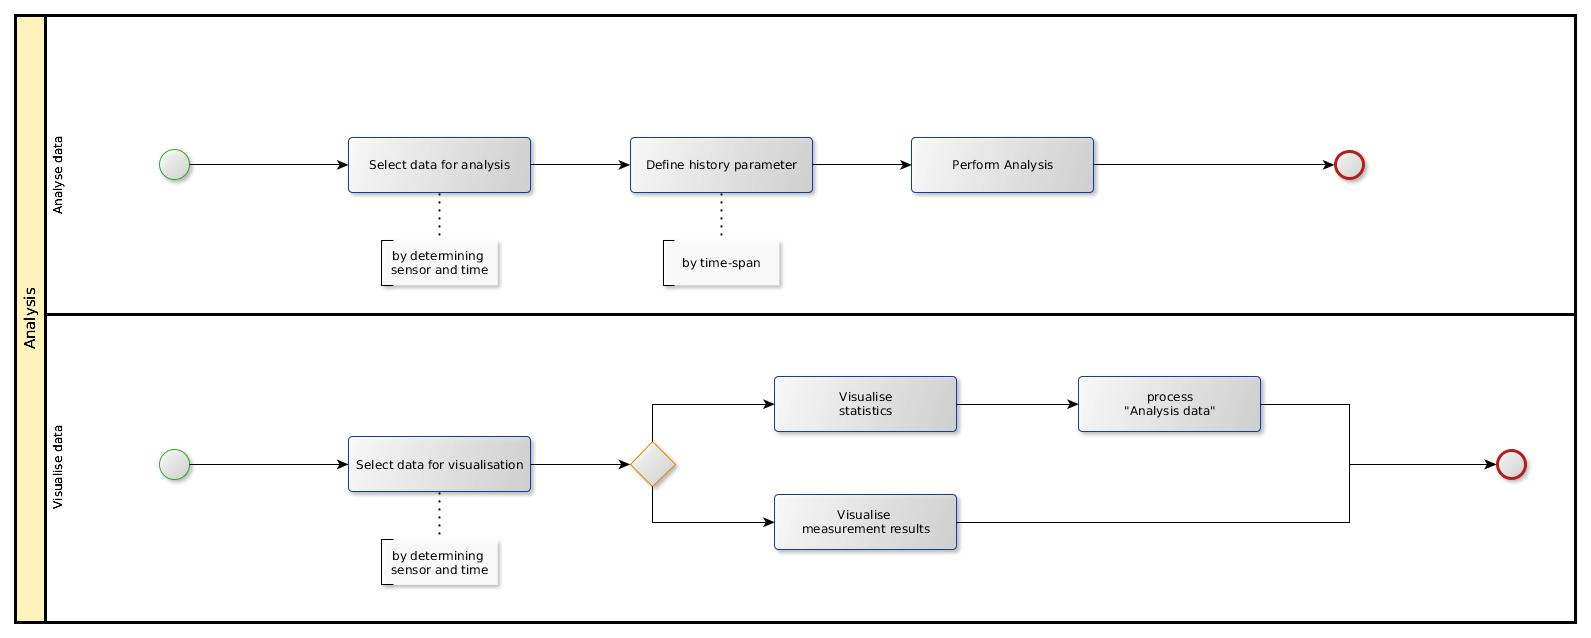
\includegraphics[scale=0.24]{graphics/bpmn_use-cases_analysis.jpg} 
	\caption{BPMN (Business Process Model and Notation) Model of the use cases describing central analysis proceedings. By F. H. Euteneuer 2013}
	 \label{fig:bpmn_use-case_analysis}
\end{figure}


\section{Product functionalities}
This part will describe the non-functional requirements of the system. This can be understood as a description of where the system will operate and how the software will operate. Non-functional requirements are requirements on a system which are not a technical functionality but a feature of the system.

The following list is describing those non-functional requirements:

\begin{description}
\item[portability] Since the system will be based on mobile devices, and those are not in any case running under windows, the software will be platform independent. Nevertheless also a web-based system is not possible, because the necessary internet connection will not be permanently available in field.
\item[performance] As described in the point before, the system will use different mobile platforms. Those do not have a hardware with a hight performance. Therefore the systems mobile part will be planed for a low performance.
\item[simplicity] The system will be used from field engineers which are working often under lots of negative influences of the environment. The system will be constructed as simply as possible to avoid unnecessary time costs for searching the right systems functionality.

\end{description}


\part{Methoden}
\chapter{Werkzeuge}
In den nachfolgenden Kapiteln gebe ich detaillierte Informationen zu den möglichen und alternativen Bausteinen für das geplante System. Die Informationen sollen der besseren Verständlichkeit des Softwaredesigns und der verwendeten System-Architektur dienen. Da mein Lösungsansatz nur ein Möglicher und keinesfalls der Einzige ist, dienen die Informationen auch dazu die Funktionsweise des Prototypen zu verstehen und kritisch zu beurteilen.

\section{Bauwerksüberwachung}
In der Einleitung wurde bereits beschrieben, wozu dieses System dienen soll, und was unter der Überwachung von Bauwerken zu verstehen ist. Anders als bei den bereits weit verbreiteten Sensortechniken, die der Überwachung von relativ kleinen technischen Objekten dienen, müssen bei der Überwachung von Gebäuden die Sensoren an teilweise sehr schwer zugänglichen und voneinander weit entfernten Positionen angebracht werden. Die Wahl einer Technologie die für die Kommunikation die bereits bestehende Infrastruktur des Internets nutzen kann umgeht das Problem komplizierter Verkabelungen.

\subsection{Sensortypen}
\subsubsection{manuelle Sensoren}
\subsubsection{automatische Sensoren}
\subsection{Relevante Eigenschaften}

\section{Entscheidungs-Unterstützung}

\section{Sensornetzwerke}
Diese Arbeit beschreibt ein System, das die Arbeit mit einem Netzwerk aus Sensoren organisieren und vereinfachen soll. Sensornetzwerke sind räumlich verteilte Sensoren die miteinander verbunden sind und über einen Computer gesteuert werden können \citep{botts_ogc_2008}. Der Grund warum Sensoren in einem Netzwerk organisiert werden sollten liegt darin, dass so Datenströme gebündelt werden können, die Messdaten durch eine Homogenisierung der Datentypen vergleichbar gemacht werden und der Wartungsaufwand für das Komplettsystem verringert wird, siehe auch \citep{resch_standardisierte_2012} \citep{bermudez_ogc_2011}. Werden Sensoren in einem Netzwerk organisiert, übernimmt die Aufgabe des Messens eine Software die den Sensor fernsteuert. Klassischerweise gehört dazu das Messen selbst, das Speichern der Daten und gegebenenfalls die Auswertung der Daten und damit verbunden eine mögliche Ereigniserkennung. Arbeitsabläufe, die für diese Arbeit von Belang sind, wurden in den Anforderungen zu Beginn der Arbeit bereits detailliert beschrieben. 

Im Englischen wird oft auch der Begriff des ``Sensor Web'' verwendet, dessen Bedeutung über die des Sensornetzwerkes (englisch ``Sensor Network'' hinaus geht. Um die beiden Begriffe eindeutig voneinander zu unterscheiden werde ich im Folgenden von Sensornetzwerken und von einem Sensor-Web sprechen. Das Sensor-Web besteht aus Sensoren die ebenfalls miteinander verbunden sind, aber auch über das Internet erreichbar sind. Das Sensor-Web stellt somit eine Erweiterung des bloßen Netzwerkes dar, weil über das Internet Sensoren verschiedener Netzwerke miteinander verbunden werden können. Die erfassten Daten der Sensoren werden über das Internet verfügbar gemacht und können über Standard Protokolle oder einer sogenannten \newacronym{API}{API}{Application Programming Interface, deutsch: Programmierschnittstelle} \gls{API} abgerufen werden \citep{broring_new_2011}\citep{botts_ogc_2008}\citep{guinard_towards_2009}.

Das Sensor Web kann als Kommunikationsebene zwischen den Sensoren und der die Daten nutzenden Software gesehen werden. Abbildung \ref{fig:swe_layer-stack} zeigt die einzelnen Ebenen der Architektur und sortiert in dem Zusammenhang häufig genannte Begriffe ein. In der Sensor Ebene ist die eigentliche Sensor Hardware organisiert. Die Kommunikation mit den Nutzern der Systeme findet sich in der Applikations Ebene.

\begin{figure}[H]
	\centering
 	 \includegraphics[scale=0.3]{graphics/SWE_layer-stack.jpg} 
	\caption{Ebenen des Sensor Web und Einsortierung von relevanten Begriffen nach \citep{broring_new_2011}}
	 \label{fig:swe_layer-stack}
\end{figure}

Noch weiter ging Kevin Ashton als er 1999 erstmals den Begriff des Internet der Dinge (englisch: ``Internet of things\") verwendete. In seiner Präsentation 1999 zum Thema \newacronym{RFID}{RFID}{Radio-Frequency Identification} \gls{RFID} bei Procter \& Gamble formulierte er eine These derzufolge in der Zukunft Computer über Sensoren ohne die Mithilfe des Menschen Informationen über die Umwelt sammeln könnten um so den Menschen zu entlasten und ihm mehr Wissen zu verschaffen als er selbst im Stande wäre. Ashton begründete dies mit der Aussage, dass das momentane Internet aus reinen Informationen besteht, Dinge wie Lebensmittel oder Brennstoffe aber wesentlich wichtiger sind, und das Internet somit auch über diese Dinge Bescheid wissen sollte \citep{ashton_that_2009}.

Das ``Web'' der Dinge wiederum ist nach \citep{broring_new_2011} eine Erweiterung des Internet der Dinge, da es gängige Protokolle für die Kommunikation zwischen realen Objekten verwendet. Funktionalitäten realer Objekte werden mittels \gls{API} über das \newacronym{HTTP}{HTTP}{Hypertext Transfer Protocol}\gls{HTTP} im Web verfügbar gemacht \citep{guinard_towards_2009}.

Sensornetzwerke spielen bei einer Großzahl der im Alltag integrierten technischen Geräte bereits eine große Rolle. In modernen Autos werden kontinuierlich Parameter wie ``Spritverbrauch'' oder Drehzahl gemessen und dann eine mögliche verbleibende Reichweite errechnet. In Computern drehen die Lüfter erst dann in einer höheren Drehzahl wenn die automatische gemessene Temperatur des Prozessors eine festgelegte stufe erreicht. Und in besonders sensiblen Geräten wie Flugzeugen findet sich eine noch viel größere Anzahl von Sensoren und auch die Auswertung der gelieferten Messerwerte wird durch komplexe Algorithmen im Cockpit für den Piloten verständlich angezeigt. Die hier aufgezählten Beispiele stellen aber jeweils ein in sich geschlossenes System dar, bei dem Datenübermittlung oder Datenmanagement "einfach" geregelt werden kann. "Einfach" soll aber nichts als technische trivial verstanden werden, sondern lediglich darauf hinweisen, dass die dafür verwendete Technologie bereits sehr weit entwickelt ist. 

Die Knoten bestehen meist aus einem oder mehreren Sensoren, einer Recheneinheit sowie der Kommunikationseinheit. Je nachdem ob die Netzwerke drahtlos oder verkabelt betrieben werden, oder ob sie einen Stromanschluss besitzen, kommen zudem noch Komponenten wie einer Antenne, oder einer Batterie dazu. Die aktuelle Forschung konzentriert sich besonders auf diese kritischen Teile der Sensorknoten. Durch den Betrieb vieler Komponenten und besonders einer drahtlosen Kommunikation wird viel Strom verbraucht, der die Operationszeit stark verkürzt. Zudem kommt, dass derart komplexe Knoten momentan noch zu teuer sind, um sie in einer größeren Menge, wie sie vielleicht erforderlich wäre, installieren zu können. Siehe dazu auch \citep{akyildiz_survey_2002}.

In Bereichen deren wissenschaftliche Ausrichtung die Überwachung von räumlich größeren Objekten ist, halten seit einigen Jahren verstärkt Sensornetzwerke Einzug (siehe hier auch die Vorstellung der Projekte in der Einleitung). Derartige Sensornetzwerke haben mit einer Vielzahl von Problemen zu kämpfen, die gerade in der großen räumliche Ausdehnung begründet ist. Dazu gehören die Stromversorgung im Feld, die Datenübertragung über große Strecken und nicht zuletzt häufig auch die Witterung welche Einfluss auf verschiedene Faktoren nimmt. In der Einleitung wurden bereits zwei Projekte vorgestellt, die sich mit dem Aufbau und dem Betrieb von Sensornetzwerken zur Überwachung des Erdkörpers befassten. Ein Anderer Anwendungsfall für Sensornetzwerke wäre zum Beispiel das Kontrollieren von Überland-Stromleitungen wie es in \citep{voigt_autarkes_2012} beschrieben wird. Probleme wie der Strombedarf oder die Datenübermittlung wurden hierbei durch technisch an die Situation angepasste Eigenentwicklungen gelöst.

Näher eingehen möchte ich auf die Besonderheiten der autonomen Sensor Netzwerke. Sensoren in autonomen Netzwerken stellen jeweils für sich einen autonomen Knoten dar. Ein zentraler Knoten der alle Sensoren Organisiert ist somit nicht notwendig. Vielmehr organisiert sich das Netzwerk selber indem die sich Knoten aktiv einbringen und Daten aktiv senden oder empfangen. Konfigurieren sich die Knoten auch selber spricht man auch von einem sogenannten ``Ad-Hoc Netzwerk''. Autonome Sensornetzwerke wurden ursprünglich für militärische Zwecke entwickelt, werde heutzutage aber auf vielfältige Art im zivilen Bereichen eingesetzt. Die immer komplexeren Anforderungen an die technische Überwachung diverser Phänomene fördert die Entwicklung von autonomen Ad-Hoc Netzwerken. Einen Vorteil, den autonome Sensornetzwerke mit sich bringen, ist die schnelle und bequeme Installation. Dadurch, dass viel Vorarbeit in die Entwicklung der Software und Hardware der Sensoren gesteckt wurde, kommt die Installation ohne manuelle Konfiguration und damit hohem Zeitaufwand aus. Von Nachteil ist allerdings, dass durch den Betrieb von zusätzlicher Hardware die aus dem Sensor einen vollwertigen Knoten machen, der Energieverbrauch meist um ein Vielfaches über dem liegt, was der Sensor alleine benötigt. \citep{voigt_illustration_2013} \citep{akyildiz_survey_2002} \citep{vieira_survey_2003} \citep{resch_standardisierte_2012}

Benjamin Voigt, siehe \citep{voigt_illustration_2013}, beschreibt in seinem Artikel unter anderem ein drahtloses Sensornetzwerk zur Überwachung eines Vulkans, dessen Zuverlässigkeit in Bezug auf die Erkennung von Ereignissen in einem zeitlich abgegrenztem Experiment untersucht wurde. Alle relevanten Ereignisse wurden zwar zuverlässig erkannt, darüber hinaus aber 99\%  nicht relevante Ereignisse. Zu den schlechten Ergebnissen führten vor Allem Fehler der Software und der Algorithmen. Das lässt den Autoren die Schlussfolgerung ziehen, dass solch ein System noch nicht für den operativen Dienst verwendbar ist. Hauptsächlich auch deshalb, weil die Lösungsansätze (höherer Betreuungsaufwand) bei Netzwerken mit einer realistischen Anzahl von Knoten (<1000) nicht finanzierbar wären.

Ein weiteres Beispiel für autonome Sensornetzwerke wäre ein Teil des in der Einleitung beschriebenen Projektes \gls{SOSEWIN}. Wie bereits beschrieben wird geplant die bestehenden Netzwerke durch ein Netzwerk aus autonom agierenden Sensoren gerade im städtischen Bereich zu erweitern. Dadurch dass die autonomen Sensoren ohne besonderes Fachwissen installiert werden können, sind auch Privatmenschen in der Lage Sensoren zu erwerben und zu betreiben, und damit zum Schutz der Gemeinschaft vor Katastrophen beizutragen.

\subsection{OGC Sensor Web Enablement}
Das \newacronym{SWE}{SWE}{Sensor Web Enablement} \gls{SWE} ist eine Initiative des \newacronym{OGC}{OGC}{Open Geospatial Consortium} \gls{OGC} und beinhaltet die Beschreibung verschiedener Standards zur Vernetzung von Sensoren im Web \citep{botts_ogc_2008}\citep{bermudez_ogc_2011}. Das \gls{OGC} ist die weltweit größte Organisation die sich um die Standardisierung des Datenverkehres von räumlichen Informationen bemüht. Das \gls{SWE} dient nicht nur zur Verknüpfung von Sensoren und zum Aufbau eines Netzwerkes, sondern es ermöglicht, Sensoren in das Web zu integrieren. Die Architektur des \gls{SWE} beinhaltet Lösungen um Sensoren im Web zu finden und zu beschreiben, um die gemessenen Daten zu lesen und um die Sensoren zu steuern \citep{botts_ogc_2008}\citep{broring_new_2011}. Das \gls{OGC} \gls{SWE} bietet mit seinen einzelnen Bausteinen des Sensor Web folgende Funktionalitäten:

\begin{description}
\item[Finden] Im Englischen steht der Ausdruck ``Discover'' für die gesamte Tätigkeit rund um das Suchen und Finden von Daten im Web. Diese Funktionalität soll das Finden der Messdaten und der Sensoren ermöglichen und vereinfachen.
\item[Sensor beschreiben] Diese Funktion liefert Metadaten zu den Sensoren wie etwa dessen generelle Eigenschaften, Arbeitsweise und Genauigkeit.
\item[Daten holen] Üblicherweise enthalten Webservices die mit Daten arbeiten eine Funktion die englischen ``Get Daten'' benannt ist. Mit dieser Funktion werden die angeboten Daten geholt.
\item[Aufgabenplanung] Um überhaupt Messergebnisse erhalten zu können muss die Arbeit des Sensoren geplant beziehungsweise werden angewiesen werden. Dies geschieht mit Hilfe dieser Funktion.
\item[Sensor abonnieren] Diese Funktion ermöglicht es passiv alle Ereignisse die der jeweilige Sensor zu vermelden hat zu erhalten.
\end{description}

\citep{botts_ogc_2008}\citep{broring_new_2011}

Die Standardisierung von Austauschprotokollen, Datentypen und Beschreibungssprachen ermöglicht es räumliche Daten einfacher und plattformübergreifend über das Web zu verbreitet und vereinfacht zu nutzen. Einzelne Standards des \gls{OGC} wurden bereits als \newacronym{ISO}{ISO}{International Standardisation Organisation} Standard eingetragen. Dadurch wird eine weltweit einheitliche Verfügbarkeit von Sensordaten gefördert. Auch andere Organisationen oder Initiativen die sich um Standardisierung von Geodaten bemühen orientieren sich an den Standards des \gls{OGC} und tragen damit zu einer Harmonisierung der Geoinformations Technologie bei. Das \gls{OGC} wiederum bemüht sich ebenfalls um ein Harmonisierung seiner eigenen Standards mit anderen wie zum Beispiel der IEEE 1451 ``Smart Transducer'' Standard Serie \citep{botts_ogc_2008}. Im Rahmen der \gls{SWE} Initiative wurden folgende Standards entwickelt:

\begin{description}
\item[Observation \& Measurement Schema] Der \newacronym{OM}{OM}{Observation and Measurement}\gls{OM} Standard beschreibt eine spezifische Vorgehensweise bei Messen von Objekteigenschaften. Diese Vorgehensweise kann -und soll- bei einer großen Bandbreite von Untersuchungen angewendet werden. Das Schema ist ein \newacronym{GML}{GML}{Geographic Markup Language}\gls{GML} Anwendungsschema für Beobachtungs- und Messdaten und ist daher geeignet um Daten in vergleichbarer Form auszutauschen und darzustellen \citep{kraak_what_2005}. Eine Beobachtung (englisch: Observations) wird im Rahmen dieses Schemas als Ereignis beschrieben dessen Ergebnis mit einem numerischen Wert ein Phänomen beschreibt. Dabei werden Beobachtungen immer einem bestimmten Objekt des Interesses und der verwendeten Methode zugeordnet. Siehe auch \citep{cox_observations_2011}.
\item[Sensor Model Language] Die \newacronym{SensorML}{SensorML}{Sensor Model Language}\gls{SensorML} dient der einheitlichen Beschreibung von Sensoren und Prozessen. Diese \gls{SensorML} Dokumente sind notwendig um die Eigenschaften der Sensoren im Web eindeutig zu beschreiben und dienen dazu die Sensoren im Web besser zu finden. Sie enthalten unter Anderem Angaben über Position, Arbeitsweise und generelle Eigenschaften der Hardware. Die Arbeitsweise eines Sensoren wird detailliert mit Eingangswerten, Ausgangswerten, Parametern und Methoden beschrieben und dient dazu besser nachvollziehen zu können wie die Messerergebnisse zustande kommen. Ein Beispiel wäre das \gls{GPS} dessen Sensoren intern bereits die gemessenen Werte (Zeitangaben über Signal-Laufzeiten) prozessieren um sie überhaupt verwendbar zu machen. Siehe auch \citep{botts_opengis_2007}.
\item[Transducer Markup Language] Die \newacronym{TransducerML}{TransducerML}{Transducer Markup Language}\gls{TransducerML} dient als Protokoll dem Austausch von Informationen zwischen der Hardware und dem Sensor Web. Der deutsche Übersetzung ``Energiewandler'' für den englische Begriff ``Transducer'' steht für die eigentliche Sensor Hardware. In der \gls{TransducerML} wird der Begriff ``Transducer'' für das Superset aller vorhandenen Sensoren und Bedienungselemente verwendet. 
%%%   Hier nochmal umformulieren!!!!!!!!!!!!!!!!!!!!!!!
\gls{TransducerML} Dokumente enthalten Informationen über die Sensoren, dienen aber auch dazu Messwerte in vergleichbarer Form zu speichern, unabhängig von der sie produzierten Hardware. Zusammengefasst stellt die \gls{TransducerML} ein Modell für das Bereitstellen von Echtzeitdaten zur Verfügung. Die Daten sind mit einem Zeitstempel und einer Referenz auf das sie produzierende Sensorsystem eindeutig nachverfolgbar.
\item[Sensor Observations Service] Der \newacronym{SOS}{SOS}{Sensor Observations Service}\gls{SOS} steht als Web-Dienst beziehungsweise \gls{API} zur Verfügung um die Sensoren zu verwalten und die Daten abzurufen und zu filtern. Der Dienst ist der direkte Kommunikationsweg zwischen dem Nutzer und dem System. Das Ziel das das \gls{OGC} mit dem \gls{SOS} verfolgt ist, eine einheitliche Methode zur Verfügung zu stellen mit der die Messungen aller unterschiedlicher Sensoren abgerufen werden können. Siehe auch \citep{na_sensor_2007}.
\item[Sensor Planning Service] Der \newacronym{SPS}{SPS}{Sensor Planning Service}\gls{SPS} dient ebenfalls der Kommunikation zwischen dem Nutzer und dem System. Im Grunde kann der Nutzer über den \gls{SPS} dem System Beobachtungs-Aufträge erteilen. Dabei werden mehrere Aufträge beziehungsweise die Anfragen an verschiedene Sensoren gebündelt an den \gls{SPS} übermittelt. Über den \gls{SPS} können außer dem Anfragen von Daten an sich auch vergangene Anfragen geändert, zurückgenommen oder dessen Status abgefragt werden. Zudem bietet er die Möglichkeit Informationen über weitere \gls{OGC} Webservices, welche sich auf die Daten der Anfrage beziehen, zu erhalten.
\item[Sensor Alert Service] Mit dem \newacronym{SAS}{SAS}{Sensor Alert Service}\gls{SAS} können Nutzer über Ereignisse automatisch informiert werden. Der \gls{SAS} stellt ein Interface dar, über das Sensorknoten Beobachtungen anbieten können. Der Service ist damit nicht ein klassischer Mitteilungsservice, sondern eine Kartei (englisch: ``registry'') für zur Verfügung stehende Benachrichtigungs-Angebote. Möchte ein Nutzer über Ereignisse informiert werden, meldet er sich bei dem \gls{SAS} and. Dieser leitet die Anfrage den passenden Nachrichtenserver weiter, der dann die gewünschten Benachrichtigungen versendet.  Der \gls{SAS} ist bislang noch nicht als vollwertiger Standard, sondern nur als sogenanntes ``Best Practices Paper'' von der \gls{OGC} veröffentlicht.
\item[Web Notification Services] Für den asynchronen Austausch von Informationen zwischen verschiedenen Services und dem Nutzer dient der \newacronym{WNS}{WNS}{Web Notification Service}\gls{WNS}. Besonders bei Langzeittransaktionen ist eine asynchrone Kommunikation notwendig um den Nutzer oder einem anderem Service die Möglichkeit zu bieten jederzeit einzugreifen. Der \gls{WNS} ist ebenfalls noch nicht als vollwertiger Standard, sondern nur als ``Best Practices Paper'' von der \gls{OGC} veröffentlicht.
\end{description}

\citep{botts_ogc_2008}\citep{woolf_gigas_2008}\citep{kunkel_teodoor:_2012}\citep{walkowski_sensor_2008}

Das \gls{OGC} hat mit der \gls{SWE} Initiative eine Komplettlösung geschaffen, die es ermöglicht verschiedenartige Sensoren in eine sogenannte \newacronym{SDI}{SDI}{Spatial Data Infrastructure -deutsch: Geodaten Infrastruktur-} \gls{SDI} einzubinden. Damit ist auch eine Visualisierung von Sensordaten eingebettet in andere Webservices wie etwa einem Kartenservice möglich \citep{broring_new_2011}. Nähere Informationen zum Aufbau und Interaktion zwischen den einzelnen Bausteinen des Sensor Web werden in den nachfolgenden Kapiteln zu den Themen Geodateninfrastruktur und Softwaredesign gegeben.

\subsubsection{Sensor Observation Service}
\subsubsection{Sensor Alert Service}
\subsubsection{Sensor Planning Service}
\subsubsection{Sensor Instance Registry}
\subsubsection{Sensor Observable Registry}
\subsubsection{Sensor Modelling Language}
\subsubsection{Metadaten}

\subsubsection{Existierende Lösungen}
\paragraph{$52\,^{\circ}$North}
Das Programmiergerüst (englisch: Framework) $52\,^{\circ}$North\footnote{www.52north.org} stellt eine der umfangreichsten und frei verwendbaren Implementierungen für das \gls{SWE} dar und wird unter Anderem in dem Projekt \gls{GITEWS} (siehe Einleitung) verwendet. Die Software entstand 2004 im Rahmen einer Initiative der Universität Münster\footnote{http://www.uni-muenster.de/de/} zusammen mit dem Unternehmen ``con terra GmbH''\footnote{http://www.conterra.de/index\_de.asp} und ab 2005 auch dem Institut für Geoinformationswissenschaften und Erdbeobachtung in Enschede (Niederlande) \newacronym{ITC}{ITC}{International Institute for Geo-Information Science and Earth Observation}\gls{ITC} \citep{botts_ogc_2008}\citep{kraak_what_2005}. 

Die Initiative verfolgt das Ziel eine freie und quelloffene Software für die Erfassung, Analyse und Visualisierung von Geoinformationen zu entwickeln. Quelloffen heißt, dass die Software unter den Lizenzbedingungen der \newacronym{GNU-GPL}{GNU-GPL}{GNU General Public License}\gls{GNU-GPL} veröffentlicht wurde. $52\,^{\circ}$North ist stark in die Weiterentwicklung der Standards rund um das \gls{SWE} der \gls{OGC} involviert.

\paragraph{istSOS}
Um für eine Risiko Management system in der Schweiz die Funktionalitäten der bisherigen \gls{SOS} Implementierungen zu erweitern entwickelte das schweizer Institut für Geowissenschaften \newacronym{IST}{IST}{Instituto scienze della Terra}\gls{IST} 2010 eine eigene Software mit dem Namen \newacronym{istSOS}{istSOS}{Instituto scienze della Terra Sensor Observation Service}\gls{istSOS}\footnote{http://istgeo.ist.supsi.ch/software/istsos/}. Die bereits existierenden Implementierungen, wie etwa das oben beschriebene $52\,^{\circ}$North  oder MapServer, erweitert das \gls{istSOS} System unter anderem um eine Unterstützung von unregelmäßigen Zeitreihen und enthält Mechanismen für die Qualitätskontrolle oder Messkorrekturen \citep{cannata_istsos_2013}. 

Das \gls{IST} entwickelte das System \gls{istSOS} komplett in Phython\footnote{http://www.python.org/} und vertreibt die Software ebenfalls unter den Lizenzbedingungen der \gls{GNU-GPL}. Das System basiert auf einem Apache Webserver\footnote{https://tomcat.apache.org/} und stützt sich auf das räumliche Datenbanksystem PostgreSQL-PostGIS\footnote{http://postgis.net/}. Neben dem \gls{SOS} enthält das \gls{istSOS} System den ``wa-Service'', der eine Reihe von Konfigurations- und Administrationswerkzeuge zur Verfügung stellt. Zusätzlich zu den Serverseitigen Implementierungen wurde auf Client-Seite auch die in JavaScript geschriebene Benutzeroberfläche ``wa-Interface'' geschaffen. Die Software-Architektur des Systems ist verschachtelt aufgebaut. Die Phyton Biliothek ``istsoslib'' stellt den Kern dar und ermöglicht Zugriff auf die Standard \gls{SOS} und auf \gls{istSOS} spezifische Funktionalitäten. Die Bibliothek ``walib'' ermöglicht als Zwischenschicht den Zugriff auf den wa-Service. Weitere Details zu der Software-Architektur finden sich in \citep{cannata_istsos_2013}\citep{cannata_istsos:_2010}.

\begin{figure}[H]
	\centering
 	 \includegraphics[scale=1]{graphics/istSOS_consumer-producer.png} 
	\caption{Interaktion mit dem istSOS System dargestellt mit einem UML Sequenzdiagramm jeweils für einen Datenkonsumenten und einen Datenproduzenten \citep{cannata_welcome_2014}}
	 \label{fig:istsos_consumer-producer}
\end{figure}

Wie bei den meisten \gls{OGC} Services wird auch mit dem \gls{istSOS} über den Austausch von standard Nachrichten über das \gls{HTTP} Protokoll kommuniziert. Die  \ref{fig:istsos_consumer-producer} zeigt sowohl für den Datenkonsumenten als auch für den Datenproduzenten Anfragen an den Service die mindestens in einer \gls{SOS} Implementierung enthalten sein müssen. Die Nachrichten werden beispielsweise mittels ``HTTP POST'' an den Service übermittelt, und dieser sendet die Antwort in Form von \newacronym{XML}{XML}{Extensible Markup Language}\gls{XML}. 

\section{Dateninfrastruktur}
\subsection{Datentypen und Datenformate}
\subsubsection{Keyhole Markup Language}
\subsubsection{Geographic Markup Language}
\subsection{Geodateninfrastruktur}
\subsubsection{Web Map Service}
\subsubsection{Web Feature Service}
\subsubsection{Web Catalogue Service}

\section{Analysemethoden}
\subsection{Methode der finiten Elemente}
\subsection{Datenkonsistenz}

\section{Mobile Dienste}
In der Einleitung bin ich bereits umfangreich auf die besonderen Charakteristiken von mobilen Diensten eingegangen, insbesondere auf die nicht-funktionellen Eigenschaften. In diesem Kapitel skizziere ich die aktuellen Forschungen in diesem Bereich und gehe detailliert darauf ein welche Rolle sie für diese Arbeit spielen können.

Der bereits zitierte Martin Breunig, siehe \citep{breunig_entwicklung_2003}, wies bereits früh auf das Potential von Geographischen Informationen für mobile Dienste hin. Die wesentlichen Teile eines solchen Systems haben sich bis heute kaum verändert, deren heutiger Entwicklungsstand ist jedoch seit dem um einiges weiter fortgeschritten. Breunig beschreibt ebenfalls die Nutzung von standardisierten Schnittstellen (siehe Kapitel Dateninfrastruktur), die besonderen Anforderungen der System-Architektur sowie die Datenvisualisierung als Kernpunkte eines Konzeptes für ein mobiles System.


\chapter{Softwareentwurf}


%\section{relevant studies}
%\input{studies}

%\section{Expected Results}
%As an overall output an demonstrating prototype of the system will be developed based on one concrete example. Most open questions will in the end be answered and evaluated, based on the developed prototype.\\
The demonstrating example will contain data from different sensors like Levelling Instruments, Total Stations and possibly also data from Accelerometers and other permanent observation sensors or Terrestrial Laser Scanners.\\
The data will be transferred to a central database in such a quality and short interval that a direct and continuous observation of changes in the measurements on a mobile device can be done.\\
On the structural health monitoring test side for this prototype, experiments should be part of the evaluation of the developed system. Such experiments like observation of loading test on the monitored construction (e.g. a bridge). \\
Changes in the measured data should be illustrated in a practicable way. An interpretation of numeric results by the user is not an option. Better would be a graphical symbolisation of changes and it pre-evaluation. What kind and which statistical interpretation of the measurements will be part of the algorithms will not be part of the development of this prototype and should be offered by the partnered scientists or parallel master thesis.\\
This master thesis will simply develop the technological structure as a basis for any implementation of adjustment and statistical evaluation algorithms.\\

%
%\section{Expected Problems}
%With the implementation but also with the theoretical questions several problems could occur.\\
First of all the biggest problem would be if there are no data for any testing available. Either due to the fact that there is not an appropriate project taking place or because of data-rights problems.\\
The possibility of a cooperation with the 'IGG Students Project' of the winter term 2013/14 might be a proper data source.\\
If there is a fitting project willing to provide its data, the used sensors might not be able to connect to the Web, and therewith one important part of the developed System cannot be tested of even worse not been developed.\\
For the streaming aspect of the System it is important that the used data are small enough for a time efficient sending via the web. In case of e.g. raw-data from TLS this would not be the case. The usage of preprocessing the data in the field and sending only intermediate results (in form of e.g. gml-geometries) might solving this problem, but errors in the necessary algorithms are invoking new problems.\\
Since the full system is depending on a database which should be given by previous work, one big problem could occur when the design of the database is inefficient for the planned tasks, or when the design is covering the full bandwidth of data the System is going to handle.\\
In the end the system will run on mobile devices. Up to now there have been three platforms established on the Smartphone and Tablet-PC marked: Googles Android, Apples iOS and Microsofts Windows. The development in context of this master thesis will at the most consider only on of these operating systems as a testing platform. The problem here would be a incompatibility to some existing platforms.


% -------------------
% ---Akronyme	 ---
% -------------------
% Acronyms



% -------------------
% --- References	 ---
% -------------------
\pagebreak
\bibliographystyle{plainnat}
\bibliography{references}{}

\end{document}
